\documentclass[tikz,border=10pt]{standalone}
\usepackage{amsmath}
\usetikzlibrary{angles,quotes}
\begin{document}
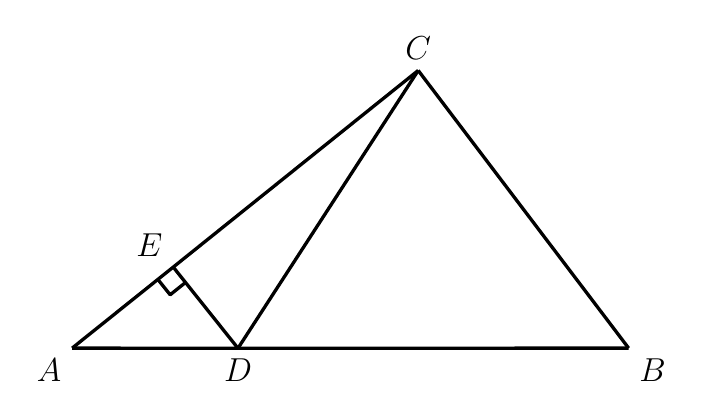
\begin{tikzpicture}[line width=1.2pt, line join=round]
\coordinate (A) at (-3.543,-1.760);
\coordinate (B) at (3.524,-1.760);
\coordinate (C) at (0.852,1.766);
\coordinate (D) at (-1.437,-1.762);




\coordinate (E) at (-2.259,-0.731);

\draw (A) -- (D) -- (B);

\draw (A) -- (E) -- (C);

\draw (B) -- (C);
\draw (C) -- (D);
\draw (D) -- (E);


\draw pic[draw, angle radius=0.250cm, line width=1.2pt] {right angle=A--E--D};


\node[below left] at (A) {\fontsize{12}{14.4}\selectfont $A$};
\node[below right] at (B) {\fontsize{12}{14.4}\selectfont $B$};
\node[below] at (D) {\fontsize{12}{14.4}\selectfont $D$};
\node[above] at (C) {\fontsize{12}{14.4}\selectfont $C$};
\node[above left] at (E) {\fontsize{12}{14.4}\selectfont $E$};
\end{tikzpicture}
\end{document}